\documentclass[tikz,border=10pt]{standalone}
\usetikzlibrary{angles}
\begin{document}
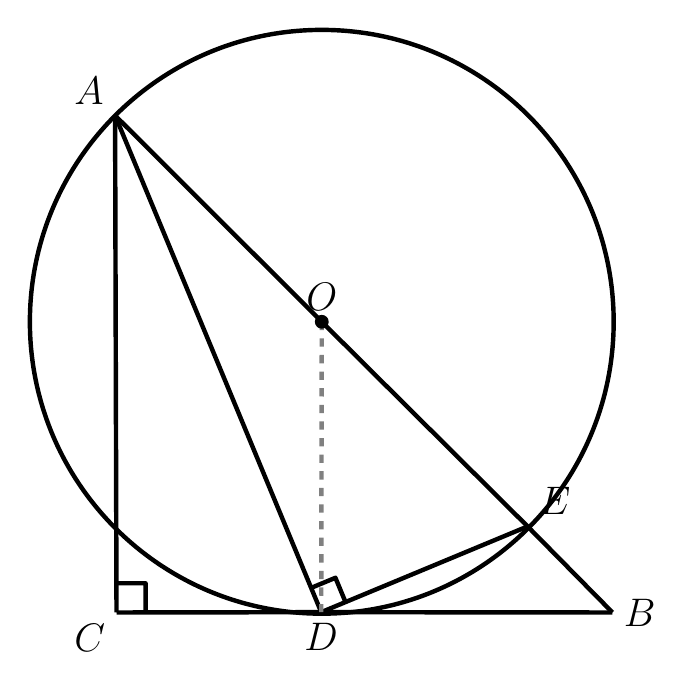
\begin{tikzpicture}[line width=1.6pt, line join=round]
\coordinate (A) at (-3.011,2.967);
\coordinate (B) at (3.306,-3.345);
\coordinate (C) at (-2.993,-3.345);
\coordinate (D) at (-0.393,-3.341);
\coordinate (E) at (2.228,-2.252);
\coordinate (O) at (-0.386,0.347);




\draw (O) circle[radius=3.707];


\draw (A) -- (O);
\draw (O) -- (E);
\draw (E) -- (B);


\draw (A) -- (C);
\draw (C) -- (D) -- (B);
\draw (A) -- (D);
\draw (D) -- (E);


\draw[dashed, gray] (O) -- (D);


\draw pic[draw, angle radius=0.371cm] {right angle=A--C--B};
\draw pic[draw, angle radius=0.334cm] {right angle=A--D--E};


\fill (O) circle (2.500pt);


\node[above left]  at (A) {\fontsize{14}{16.8}\selectfont $A$};
\node[above]       at (O) {\fontsize{14}{16.8}\selectfont $O$};
\node[above right] at (E) {\fontsize{14}{16.8}\selectfont $E$};
\node[right]       at (B) {\fontsize{14}{16.8}\selectfont $B$};
\node[below left]  at (C) {\fontsize{14}{16.8}\selectfont $C$};
\node[below]       at (D) {\fontsize{14}{16.8}\selectfont $D$};
\end{tikzpicture}
\end{document}